\section{CCF}
One example of service, that can be added on a cloud to make it confidential is the Confidential Consortium Framework (CCF) \cite{Howard}. It wants to guarantee the CIA requirements (confidentiality, integrity and availability) on multiparty applications.
\subsection{Idea}
%TODO: graphic of figure 2 in ccf paper
The basic idea of CCF is that one or more users can access 
\begin{figure}[h]
	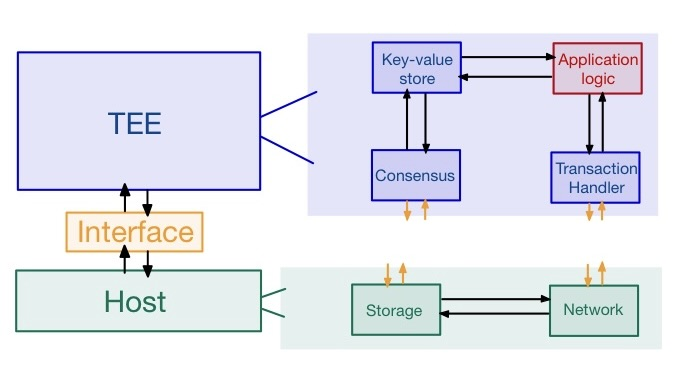
\includegraphics[scale=0.35]{pictures/basic_ccf}
	\caption{Basic CCF description}
	\label{cia}
\end{figure}
\subsection{Confidentiality}
\subsection{Reconfiguration}
\subsection{Desaster Protocol}
\subsection{TCB}
\subsection{Challenges}
As mentioned before CCF does not have a rollback detection, because it allows rollback attacks to happen, because it is not affecting the system. The problems are that they (1) make the assumption that the code inside the TEE cannot be changed and (2) that thy put their persistent storage outside the TEEs and is therefore not protected for a rollback attack.